\documentclass[a4paper,12pt]{article}

\title{Biology 30 IB \\ Cells, Chromosomes, \& DNA}
\author{Jad Chehimi}

% document setup
\renewcommand{\familydefault}{\sfdefault}
\linespread{1.25}
\usepackage[margin=1in]{geometry}
\usepackage{setspace}
\usepackage{enumitem}
\setlist{nosep}
\usepackage{amsmath}

%% highlighting
\usepackage{color,soul}

% tools
\usepackage[hidelinks]{hyperref}
\usepackage{float}
%% images
\usepackage{graphicx}
\graphicspath{ {./images/} }
%% science
\usepackage{siunitx}

\begin{document}
\maketitle

% temp
\begin{center}
\Huge
Unfinished!
\normalsize
\end{center}
% temp

\tableofcontents

\pagebreak

\section{Terms}
\begin{itemize}
    \item{\textbf{Stomatic cells} are all cells in the body \hl{except sex cells}---sperm and egg cells.}
    \item{\textbf{Cell division} is done by Eukaryotic cells---have a nucleus.}
    \item{\textbf{Binary fission} is done by Prokaryotic cells---have no nucleus, such as \hl{bacteria}.}
\end{itemize}

\section{Cell Division}
\subsection{Purpose}
\begin{itemize}
    \item{Unicellular organisms (i.e. \hl{zygote}) $\longrightarrow$ Multicellular organisms}
    \item{Growth and maintenance of body cells---\hl{replacement} of worn out cells}
\end{itemize}

\subsection{Chromosomes}
\begin{itemize}
    \item{
            Comprised of...
            \begin{itemize}
                \item{nucleic acids (DNA)}
                \item{proteins}
            \end{itemize}
        }
    \item{
            Either...
            \begin{itemize}
                \item{\textbf{Uncondensed} aka. \textbf{Chromatin} = long, thin strands. invisible to microscope}
                \item{\textbf{Condensed} = thick \& shortened. visible to microscope}
            \end{itemize}
        }
\end{itemize}

\subsection{Chromatid}
\begin{itemize}
    \item{The strand that makes up a normal chromosome.}
    \item{
            In mitosis...
            \begin{itemize}
                \item{A chromosome duplicates into two \hl{identical} chromatids, joined together by a \textbf{centromere}, to form a \textbf{duplicated chromosome}.}
                \item{These chromatids are referred as \textbf{sister chromatids} in this state.}
                \item{Each chromatid of a duplicated chromosome goes to each of the two new cells.}
            \end{itemize}
        }
\end{itemize}

\begin{figure}[H] 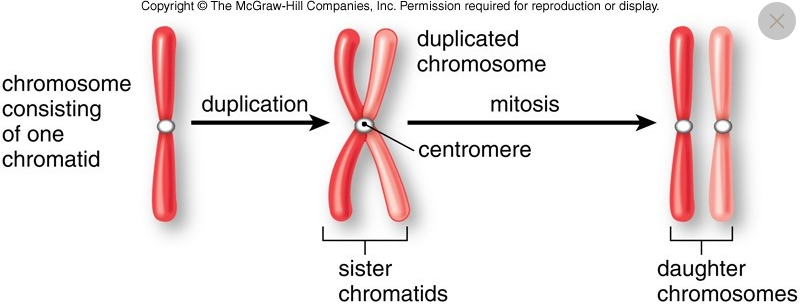
\includegraphics[width=\textwidth]{chromosome} \end{figure}

\section{Cell Cycle}
\begin{figure}[H] 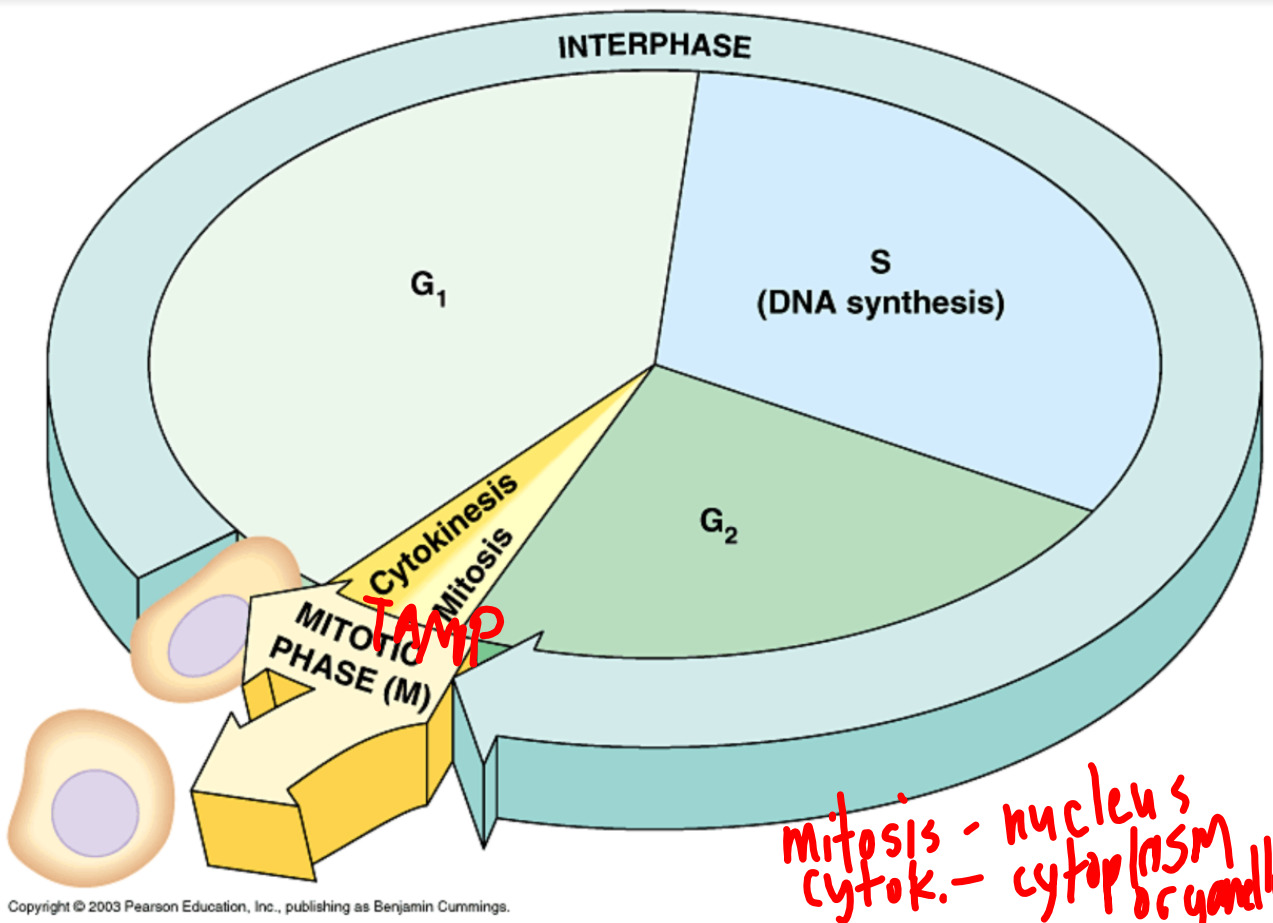
\includegraphics[width=\textwidth]{cellcycle} \end{figure}

A continuous cycle that involves all steps of a cell's life, especially cell division.

\subsection{Interphase}

\begin{itemize}
    \item{90\% of cell cycle.}
    \item{All cell activity when not dividing.}
\end{itemize}

\subsubsection{Gap 1 ($G_1$)}
\begin{itemize}
    \item{Cell growth and general function.}
    \item{After cell division, cells may be smaller than their parent. Cell growth is needed.}
\end{itemize}

\subsubsection{S Phase ($S$)}
\begin{itemize}
    \item{DNA is doubled.}
    \item{Single(-chromatid) chromosome $\xrightarrow{\textrm{duplication}}$ double(-chromatid) chromosome.}
\end{itemize}

\subsubsection{Gap 2 ($G_2$)}
\begin{itemize}
    \item{Organelles are doubled. \emph{(building proteins, new cell membranes)}}
\end{itemize}

\subsection{Mitosis}\noindent

Occurs in stomatic cells.

Distribution of \hl{nucleus and its contents}.

\subsubsection{Prophase}
\begin{itemize}
    \item{Chromatin condense---shorten \& thicken---into chromosomes, becoming visible.}
    \item{Nuclear membrane fades.}
    \item{
            Animal cells only...
            \begin{itemize}
                \item{\textbf{Centrioles} move to opposite poles of cell. (N/S, E/W)}
                \item{Centrioles deploy \textbf{spindle fibers}.}
            \end{itemize}
        }
\end{itemize}

\begin{figure}[H]
    \centering
    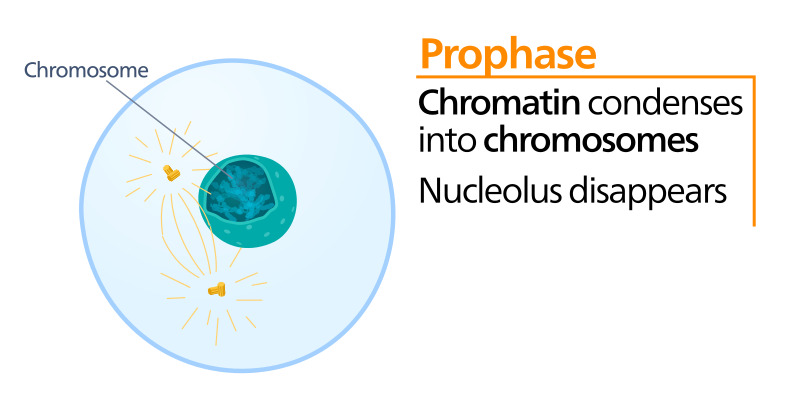
\includegraphics[width=0.5\textwidth]{prophase}
\end{figure}

\subsubsection{Metaphase}
\begin{itemize}
    \item{\textbf{Equatorial plate} = center of cell.}
    \item{Sister chromatids move towards equatorial plate.}
    \item{Chromosomes attach to spindle fibers.}
\end{itemize}

\begin{figure}[H]
    \centering
    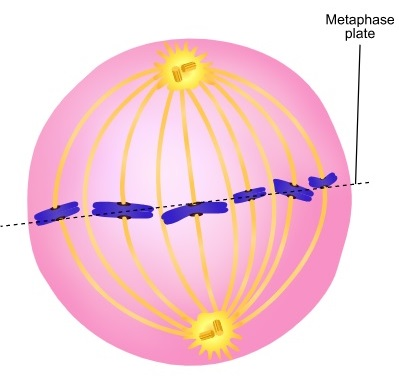
\includegraphics[width=0.5\textwidth]{metaphase}
\end{figure}

\pagebreak

\subsubsection{Anaphase}
\begin{itemize}
    \item{Centromeres divide.}
    \item{(Now) chromatids move towards spindle fibers---i.e. opposite poles of cell.}
\end{itemize}

\begin{figure}[H]
    \centering
    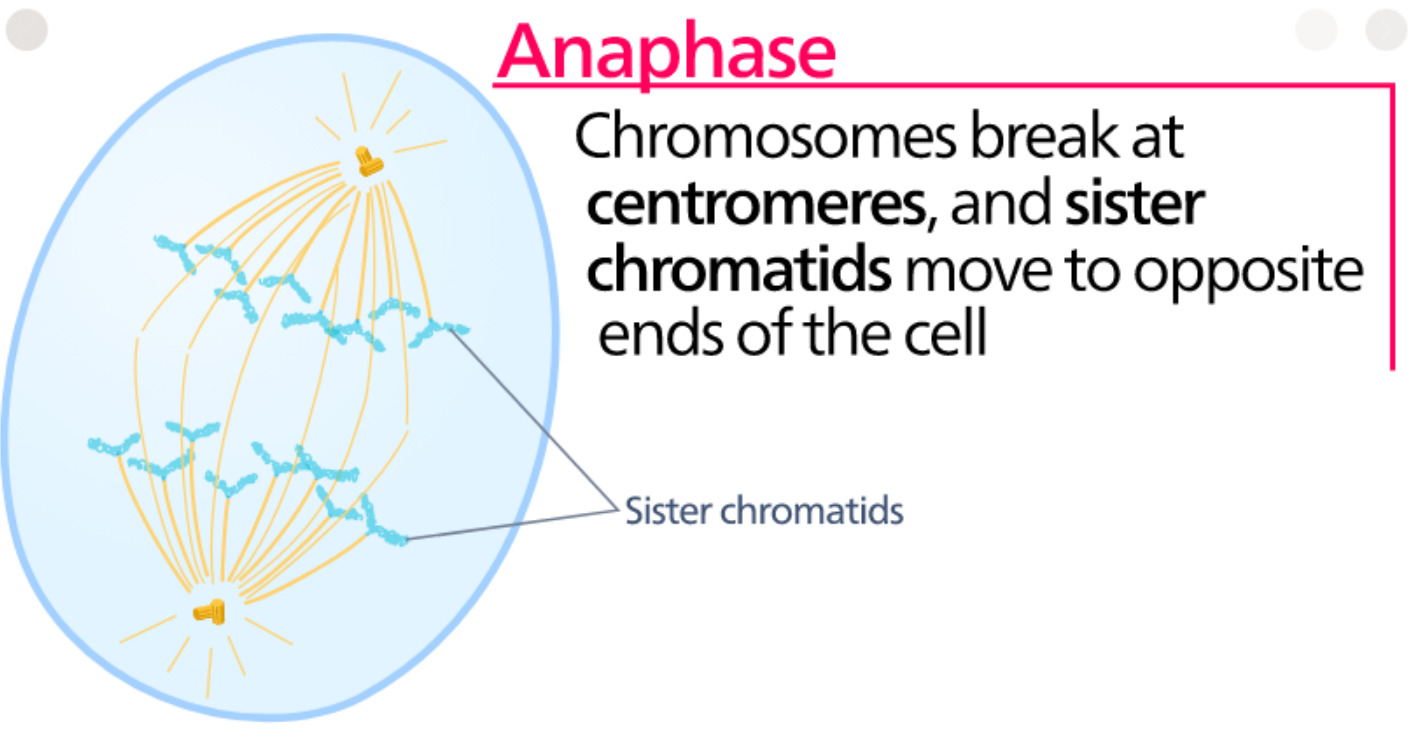
\includegraphics[width=0.75\textwidth]{anaphase}
\end{figure}

\subsubsection{Telophase}
\begin{itemize}
    \item{Spindle fibers dissolve.}
    \item{Nuclear membrane forms around each mass of chromatin.}
    \item{
            \textbf{Cytokinesis} occurs.

            \begin{itemize}
                \item{\hl{Division of cytoplasm} and \hl{distribution of organelles} to "daughter" cells.}
                \item{Involves \textbf{cleavage}, pinching off in the center as the cytoplasm moves to opposite poles.}
                \item{In plant cells only, a \textbf{cell plate} is distributed, which develops into a new cell wall.}
            \end{itemize}
        }
\end{itemize}

\begin{figure}[H]
    \centering
    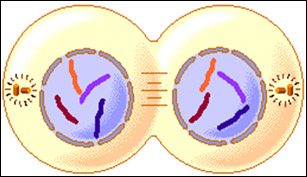
\includegraphics[width=0.75\textwidth]{telophase}
\end{figure}

\end{document}
